
\chapter{Desenvolvimento e Resultados}

Este capítulo descreve as cinco etapas de desenvolvimento do projeto proposto:

\begin{itemize}
    \item construir os \textit{datasets} de \textit{barcodes} e números;
    \item treinar e avaliar o melhor modelo de rede neural para código de barras e números;
    \item implementar o algoritmo de detecção dos código de barras;
    \item implementar o algoritmo de detecção dos números;
    \item implementar o sistema web.
\end{itemize}

A Figura \ref{fig:imagemBase} é utilizada como referência para a explicação do sistema ao longo do capítulo.

\begin{figure}[h!]
	\centering
	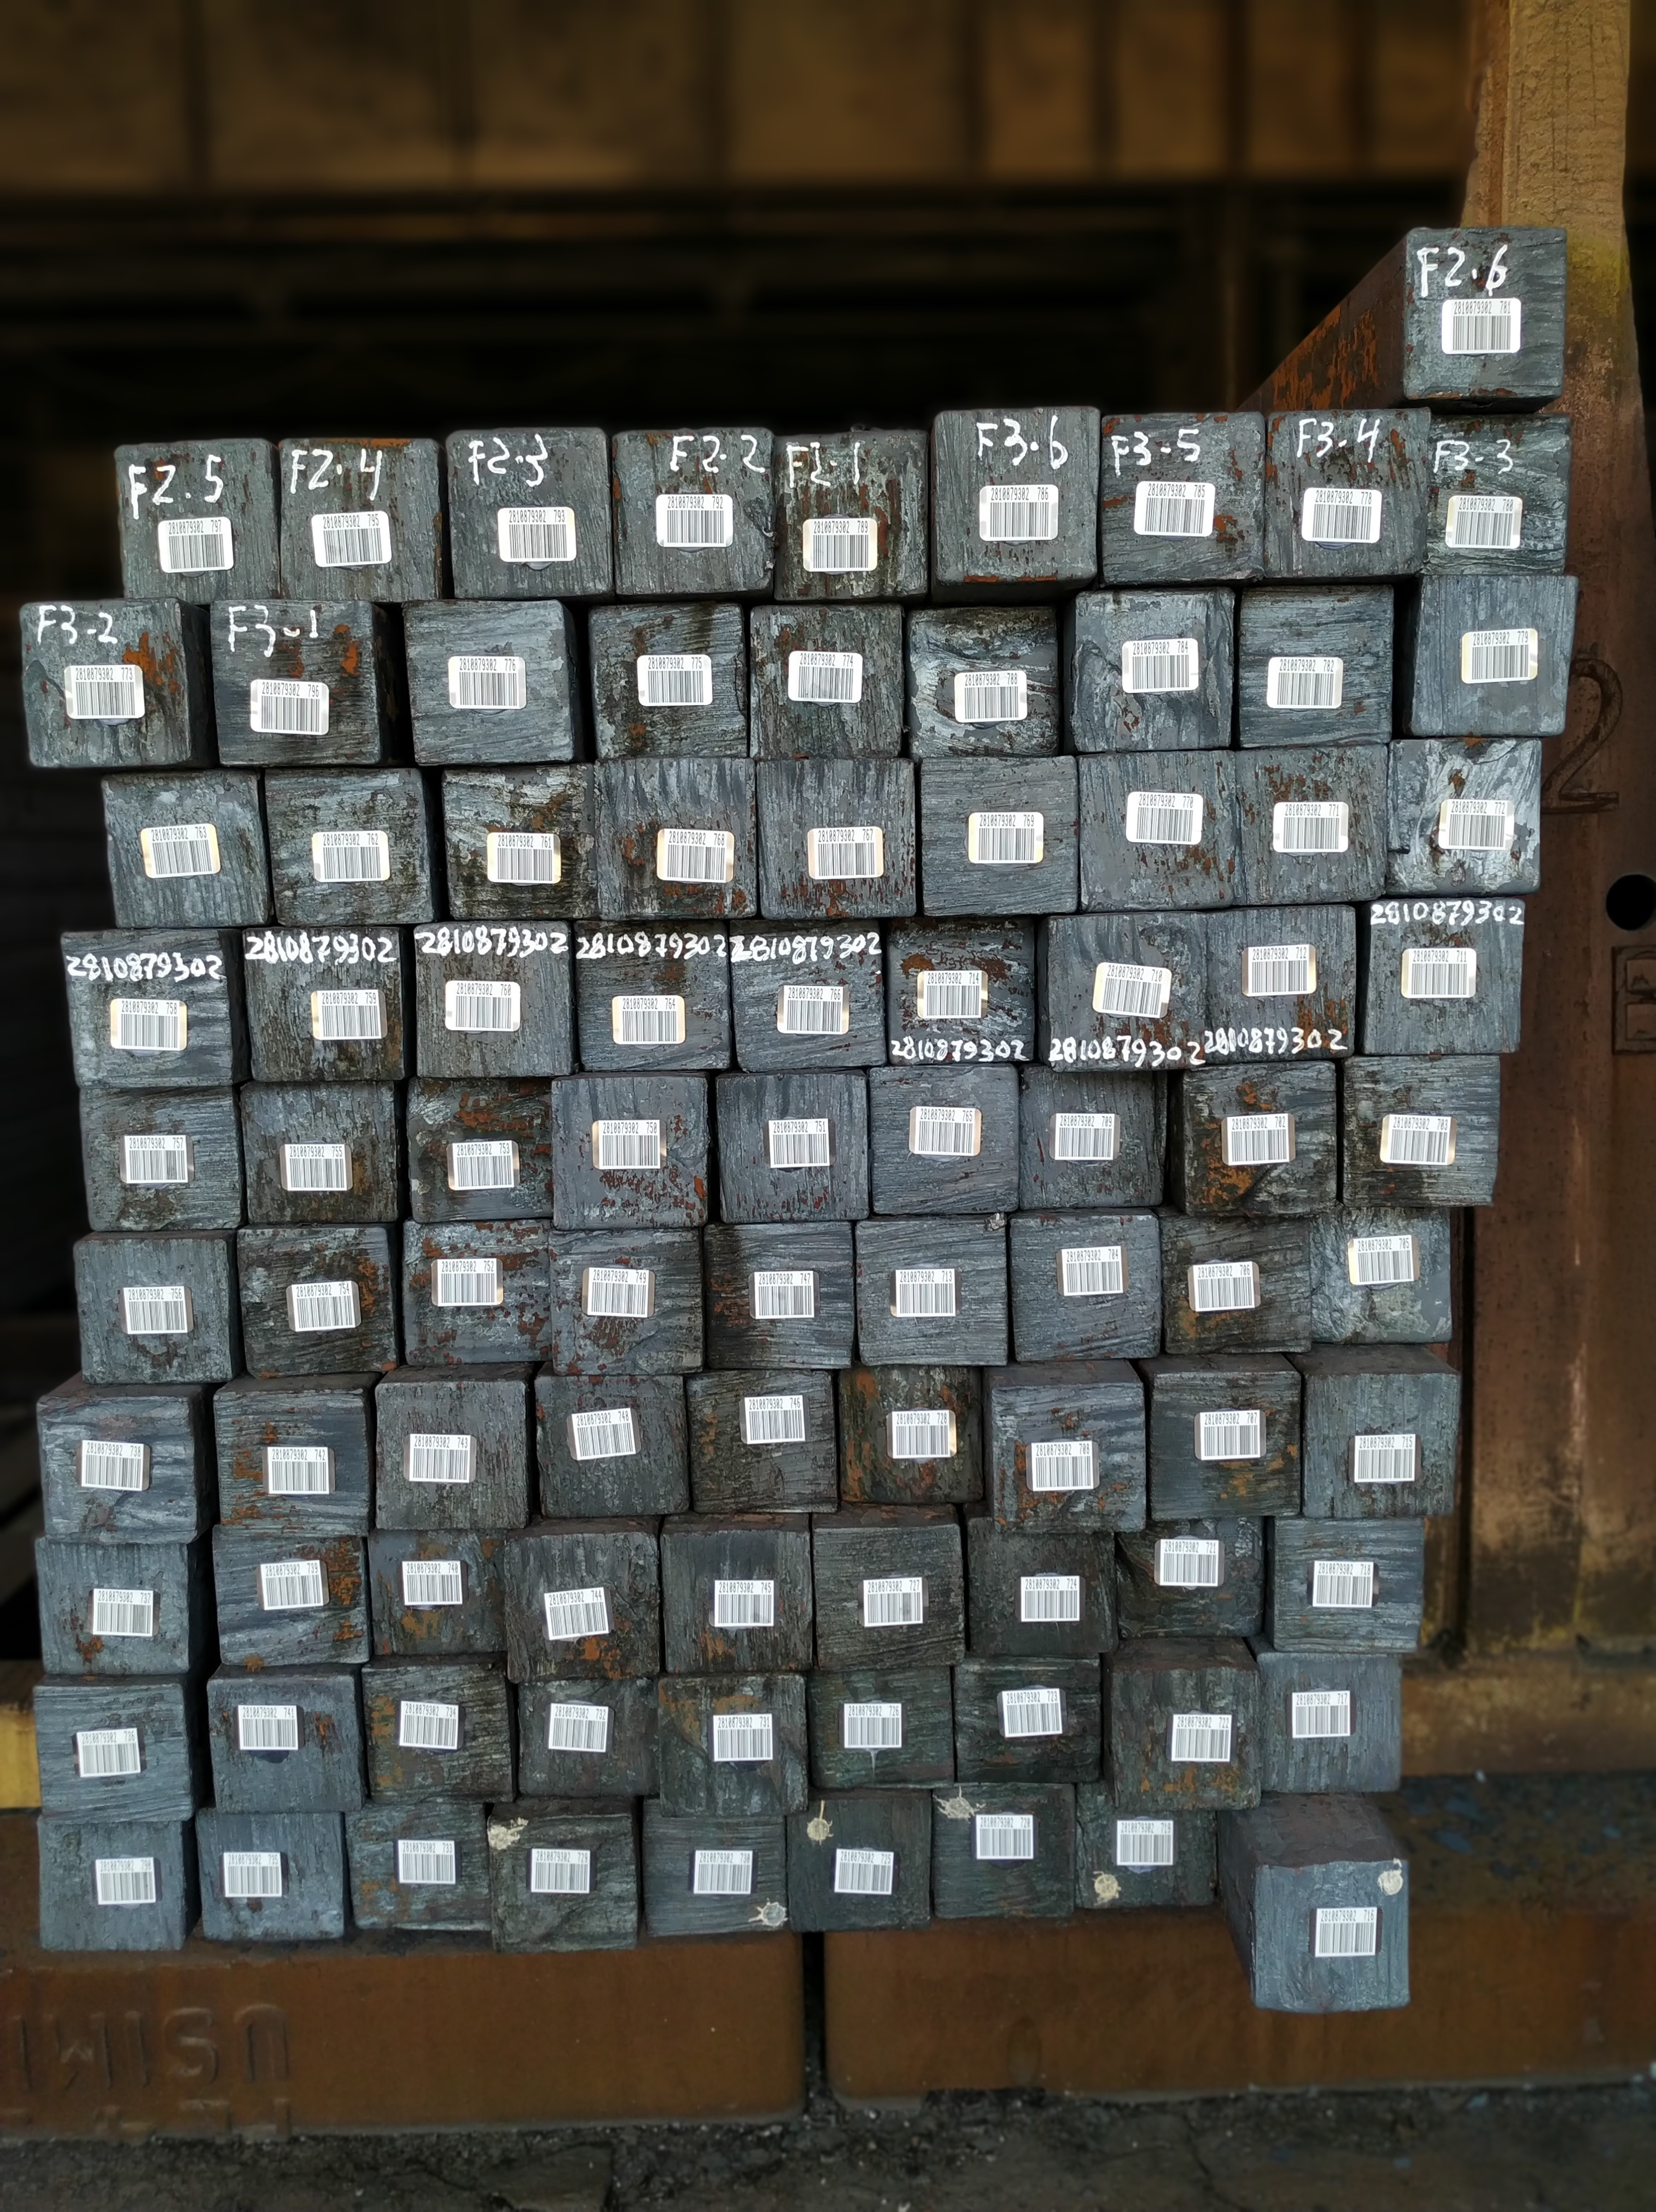
\includegraphics[width=0.5\linewidth]{figuras/img1.jpg}
	\caption{Imagem exemplo uma corrida de tarugos.}
	\label{fig:imagemBase}
\end{figure}

\section{Montagem dos \textit{datasets}}

Inicialmente foi feito o \textit{download} do conjunto de dados de \textit{barcodes} disponibilizado pelo laboratório \citeauthor{Arte-Lab}\footnote{http://artelab.dista.uninsubria.it/} com cerca de 500 imagens de código de barras para o \textit{dataset} inicial.As pastas do \textit{dataset} são criadas segundo o modelo de divisão apresentado no Código \ref{cod:folders}.

\begin{lstlisting}[caption=Divisão dos arquivos para dataset, label=cod:folders][htb!]
        +---barcode
        |   +---train
        |   |   +---annotations
        |   |   \---images
        |   \---validation
        |       +---annotations
        |       \---images
        
        +---number
        |   +---train
        |   |   +---annotations
        |   |   \---images
        |   \---validation
        |       +---annotations
        |       \---images
\end{lstlisting}

Através do método \textit{Data Augmentation} (Seção \ref{sec:dataAugm}), a base de dados foi ampliada para melhorar os resultados da rede. O modelo foi aplicado nas 500 imagens do \textit{dataset} e ao finalizar o método haviam 1263 imagens de códigos de barras na base de dados.

Com a imagem completa da corrida dos tarugos (Figura \ref{fig:imagemBase}), recorta-se manualmente as etiquetas e também aplica-se o método \textit{Data Augmentation}, gerando assim a base de dados de números. Foi escolhido utilizar os números localizados nas etiquetas após diversos treinamentos realizados com fontes numéricas diferentes que não resultaram em uma acurácia de detecção do número satisfatória (Figura \ref{fig:barcodeDataset}).

Parte das imagens, 75\%, são alocadas na pasta \textit{\enquote{/validation}}e as demais em \textit{\enquote{/train}}  tanto no \textit{dataset} de \textit{barcodes} como no de números.

\begin{figure}[H]
	\centering
	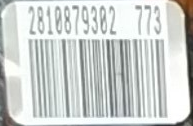
\includegraphics[width=0.25\linewidth]{figuras/MachineLearning/barcodeDataset.png}
	\caption{Montagem \textit{dataset} de números}
	\label{fig:barcodeDataset}
\end{figure}

O \textit{software} LabelImg (Subseção \ref{sub:LabelImg}) foi utilizado para fazer as anotações das imagens para que seja gerado o arquivo PASCAL VOC no formato XML (Figura \ref{fig:barNumAn}).

\begin{figure}[htbp]
	\centering
	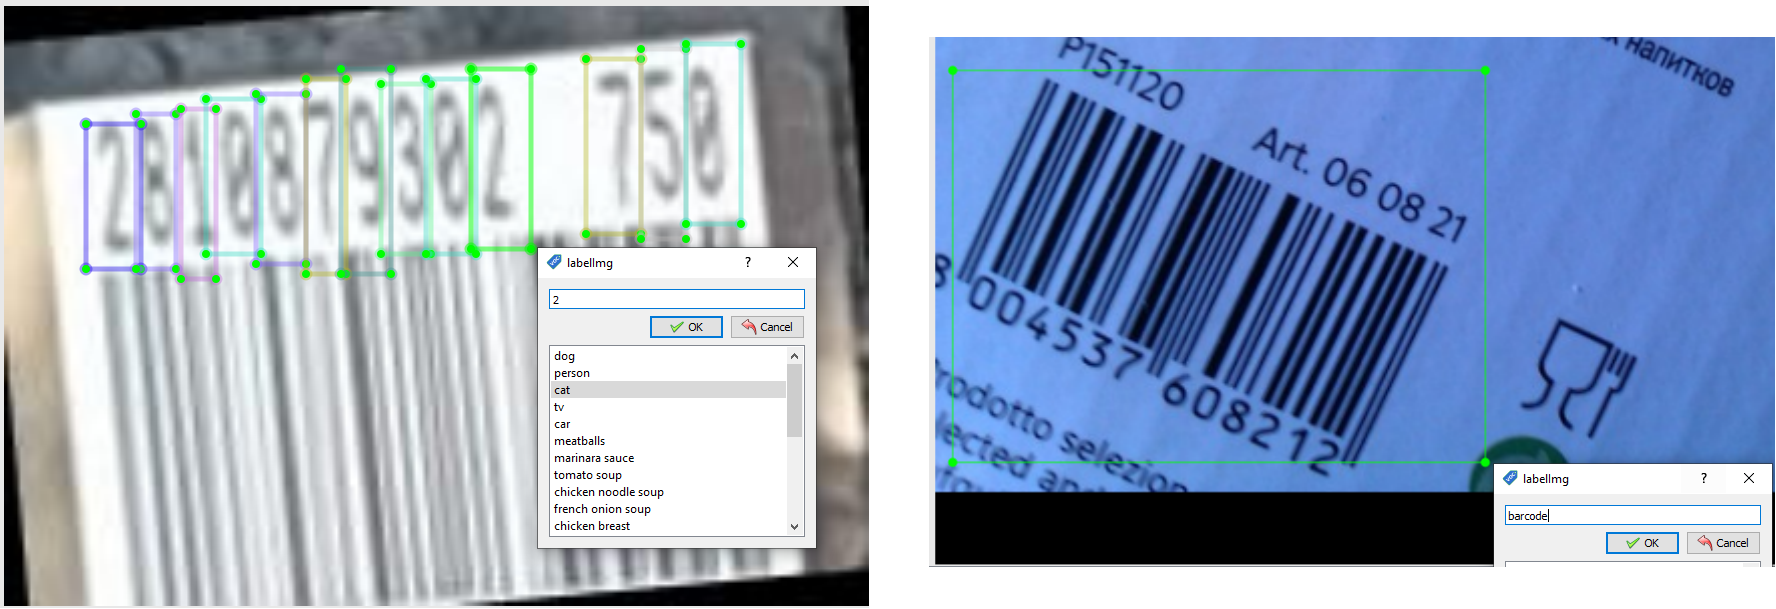
\includegraphics[width=0.9\linewidth]{figuras/MachineLearning/barNumAn.png}
	\caption{Anotações das imagens (Números e \textit{Barcodes})}
	\label{fig:barNumAn}
\end{figure}

\section{Fase de treinamento}

Nesta seção, a rede neural pré-treinada YOLOVv3 (Subseção \ref{sub:Yolov3}) treina, avalia e seleciona o melhor modelo de \textit{barcode} e número.

\subsection{Treinando o modelo}

Utilizando a biblioteca ImageAI e importando a classe \textit{DetectionModelTrainer}, o modelo é treinado da seguinte forma (Código \ref{cod:modeTrain}):
\newline
\begin{lstlisting}[caption=Exemplo de código do método \textit{data augmentation}, label=cod:modeTrain][htb!]
from imageai.Detection.Custom import DetectionModelTrainer

trainer = DetectionModelTrainer()
trainer.setModelTypeAsYOLOv3()
trainer.setDataDirectory(data_directory="barcode")
trainer.setTrainConfig(object_names_array=["barcode"], batch_size=4, 
                    num_experiments=11,
                    train_from_pretrained_model="pretrained-yolov3.h5")   
trainer.trainModel()
\end{lstlisting}

\begin{itemize}
    \item \textit{object\_names\_array}: matriz que contém os nomes dos objetos no \textit{dataset};
    \item \textit{batch\_size}: indica o tamanho do \textit{batch} para o treinamento;
    \item \textit{num\_experiments}: indica o número de vezes que a rede treinará sobre todas as imagens da base de dados.
\end{itemize}

\begin{figure}[H]
	\centering
	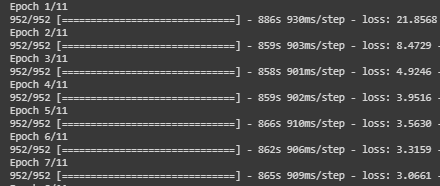
\includegraphics[width=0.7\linewidth]{figuras/MachineLearning/barcodeTraining.png}
	\caption{Exemplo de treinamento do modelo de código de barras.}
	\label{fig:barTrain}
\end{figure}

Durante o treinamento, para cada experimento, a perda total geral de validação (por exemplo - \textit{loss}: 21.8568) é relatada (Figura \ref{fig:barTrain}).
%
Após cada treinamento, se há redução do atributo \textit{loss}, um novo modelo é salvo na pasta "/barcode/models". Quanto menor o número absoluto do \textit{loss}, melhor é o modelo de um modo geral. Ele indica o quão longe está da solução "ideal". 

A função de perda ou \textit{Loss}, é um método de avaliar quão bem o modelo lida com o \textit{dataset}. Caso o modelo estiver mal treinado, o que acontece normalmente em função dos dados utilizados, sua função de perda produzirá um valor elevado. Se o modelo for muito bom, o resultado será um número menor. A medida que é alterada partes do  algoritmo para tentar aprimorar o modelo, a função de perda informa se está chegando à solução "ideal".

O método \textit{trainer.evaluateModel} mostra as métricas de saída de cada modelo e a partir dele, avaliaremos o mAP\footnote{mAP (Precisão Média) é uma métrica popular na medição da precisão de detectores de objetos.} de cada um destes modelos de detecção (Código \ref{cod:metrics}).

\begin{lstlisting}[caption=Métricas de saída do modelo, label=cod:metrics][htb!]
metrics = trainer.evaluateModel(model_path="detection_model-ex-013--loss-0003.066.h5", json_path="detection_config_barcode.json", iou_threshold=0.5, object_threshold=0.3, nms_threshold=0.5)
\end{lstlisting}

Melhores resultados encontrados de modelos de \textit{barcodes} e números aplicando a métrica de avaliação são apresentados na tabela \ref{tab:Result}:

\begin{table}[H]
	\centering
	\begin{tabular}{|l|l|l|}
		\hline
		\rowcolor[HTML]{ECF4FF} 
		\multicolumn{1}{|c|}{\cellcolor[HTML]{ECF4FF}\textit{Característica}} &
		\multicolumn{1}{|c|}{\cellcolor[HTML]{ECF4FF}\textit{Barcode}} & \multicolumn{1}{c|}{\cellcolor[HTML]{ECF4FF}\textit{Number}}\\ \hline
		\textit{Loss} & 3.066 & 12.296\\ \hline
		\textit{mAP} & 91.07\% & 77.90\%  \\ \hline
	\end{tabular}
	\caption{Resultados obtidos dos modelos de \textit{barcode} e número.}
	\label{tab:Result}
\end{table}

Ao detalhar a média de precisão dos números, observa-se a probabilidade de cada número ter sido corretamente identificado como também o mAP do modelo (Figura \ref{fig:numberTrained}). Também pode-se observar média de precisão dos \textit{barcodes}, bem como o mAP na figura \ref{fig:barcodeTrained}.


\begin{figure}[H]
	\centering
	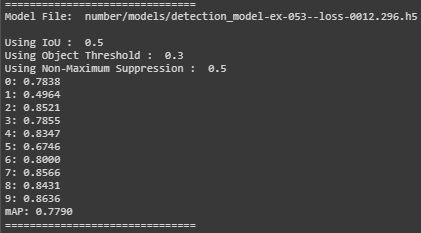
\includegraphics[width=0.7\linewidth]{figuras/MachineLearning/numberTrained.png}
	\caption{Médias de precisões dos números.}
	\label{fig:numberTrained}
\end{figure}

\begin{figure}[H]
	\centering
	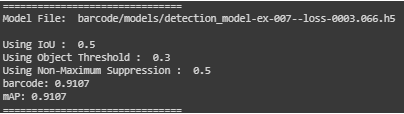
\includegraphics[width=0.7\linewidth]{figuras/MachineLearning/barcodeTrained.png}
	\caption{Médias de precisões dos \textit{barcodes}.}
	\label{fig:barcodeTrained}
\end{figure}


\section{Implementação dos algoritmos de detecção}

Nesta seção implementa-se os algoritmos\footnote{\textit{shorturl.at/bluOV}} de detecção de \textit{barcodes} e números utilizando os modelos de redes neurais treinadas na seção anterior. Para que o sistema complete o fluxo e entregue os dados ao sistema web de forma correta, serão necessários \textit{scripts} \footnote{Conjunto de instruções para que uma função seja executada em determinado aplicativo.} de criações de pastas ao longo das etapas.

A divisão de pastas do sistema de detecção foi elaborada para facilitar a comunicação entre os serviços, de acordo com as necessidades do sistema web. A Figura \ref{fig:folderSystem} representa o desenvolvimento da estrutura dos diretórios utilizados no projeto.

\begin{figure}[H]
	\centering
	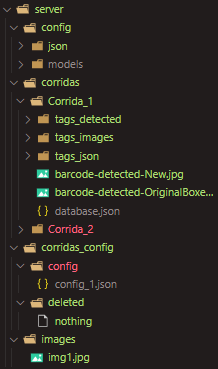
\includegraphics[width=0.4\linewidth]{figuras/MachineLearning/folderSystem.png}
	\caption{Divisão dos arquivos do sistema de detecção}
	\label{fig:folderSystem}
\end{figure}

\begin{itemize}
    \item \textbf{config}: Arquivos de configuração do sistema, como os modelos de \textit{barcode} e números e os arquivos JSON de configuração para treinar a rede;
    \item \textbf{corridas}: Pastas contendo todas as corridas;
    \begin{itemize}
        \item \textbf{Corrida\_1}
            \begin{itemize}
                \item \textbf{tags\_detected}: Imagens das etiquetas recortadas contendo as bbox dos números;
                \item \textbf{tags\_images}: Imagens das etiquetas recortadas;
                \item \textbf{tags\_json}: Arquivos  de configuração de cada etiqueta como, por exemplo, números detectados, acurácias, posições das bbox de cada número;
                \item \textbf{barcode-detected-New.jpg}: Imagem contendo as bbox aumentadas pelo script;
                \item \textbf{barcode-detected-OriginalBoxes.jpg}: Imagem contendo as bbox originais;
                \item \textbf{database.json}: Arquivo resumindo as configurações das etiquetas que se encontram na pasta "/tags\_json";
            \end{itemize}
    \end{itemize}
     \item \textbf{corridas\_config}
        \begin{itemize}
            \item \textbf{config}: Arquivos de configuração resumo de cada corrida para consumo do sistema web;
            \item \textbf{deleted}: Pasta referente às corridas deletadas pelo sistema web;
        \end{itemize}
    \item \textbf{images}: Pasta contendo todas as imagens que são \textit{input} do sistema (Ex: Figura \ref{fig:imagemBase}).
\end{itemize}


\subsection{Detecção de \textit{barcode}}

O reconhecimento dos \textit{barcodes} é essencial para a separação das etiquetas e posterior identificação dos números.
%
Inicialmente, para a detecção dos códigos de barras, são criadas funções para verificar se a mesma bbox está sendo detectada duas ou mais vezes. Para isso é feita uma função de interseção sobre união entre duas bbox, comparando cada uma com todas as outras existentes na imagem. Assim, caso seja retornado um valor da função diferente de zero, uma bbox é deletada (Código \ref{ap:IoU}).

Ao iniciar o treinamento do modelo, identificou-se que as bbox ficavam menores que as etiquetas o que levava à perda de alguns números. Para que isso não acontecesse, foi necessário aumentar, manualmente, 50 \textit{pixels} em cada bbox (Código \ref{ap:AumentaBbox}).
%
Cada imagem de bbox é salva na pasta "/tags\_images" para ser utilizada pelo modelo de detecção de números na próxima etapa (Figura \ref{fig:bboxNew}).

\begin{figure}[H]
	\centering
	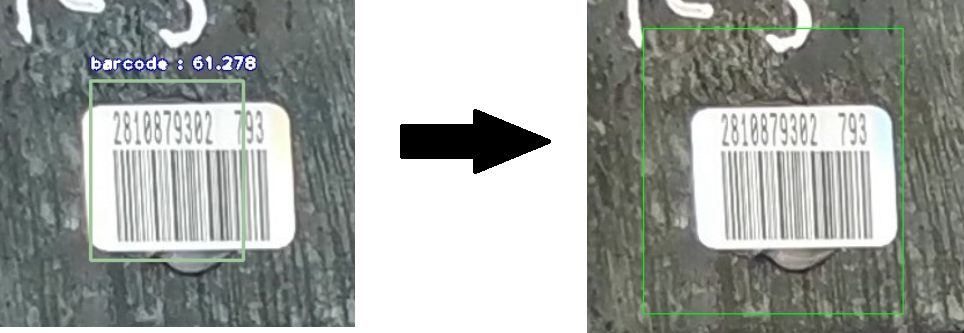
\includegraphics[width=1\linewidth]{figuras/MachineLearning/bboxNew.png}
	\caption{Resultado do aumento das bbox}
	\label{fig:bboxNew}
\end{figure}



Os resultados da saída do modelo da rede neural de \textit{barcodes} são o nome do objeto detectado, a acurácia de cada \textit{barcode} e a posição da bbox de cada código de barras (Figura \ref{fig:indentBarcodes}).

\begin{figure}[H]
	\centering
	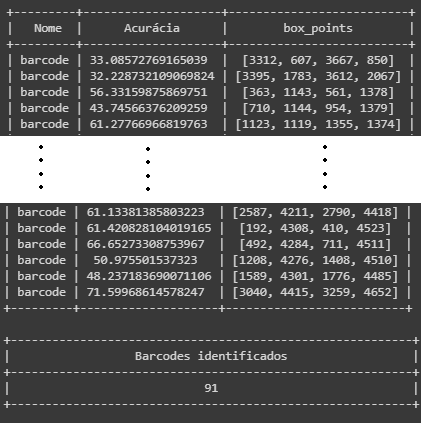
\includegraphics[width=0.6\linewidth]{figuras/MachineLearning/indentBarcodes.png}
	\caption{ Resultado do modelo de detecção de \textit{barcodes}}
	\label{fig:indentBarcodes}
\end{figure}


\subsection{Detecção de número}


O algoritmo de detecção de números utiliza as imagens localizados na pasta "/tags\_images", que foram recortadas pelo modelo anterior.
%
Tendo como referência a Figura \ref{fig:numDup}, verifica-se que mais de uma bbox abrangia um mesmo número, fazendo com que este fosse identificado repetidamente. 

\begin{figure}[H]
	\centering
	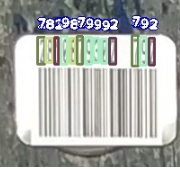
\includegraphics[width=0.4\linewidth]{figuras/MachineLearning/numDup.png}
	\caption{Etiqueta com múltiplas detecções de números}
	\label{fig:numDup}
\end{figure}

Para solucionar este problema foi preciso reconhecer quais bbox estavam superpostas. Para isso, analisando as imagens, foi identificado que dois números consecutivos, teriam seus centros distantes, pelo menos, 6 \textit{pixels} entre si. 
%
Para este cálculo foi utilizada  uma função que calcula a coordenada central de cada bbox e aplicada a equação de Distância Euclidiana\footnote{Distância entre dois pontos.} para saber o afastamento entre dois centros subsequentes.
%
A distância identificada, Dab, menor que 6 \textit{pixels} revela a repetição do número.

\begin{figure}[H]
	\centering
	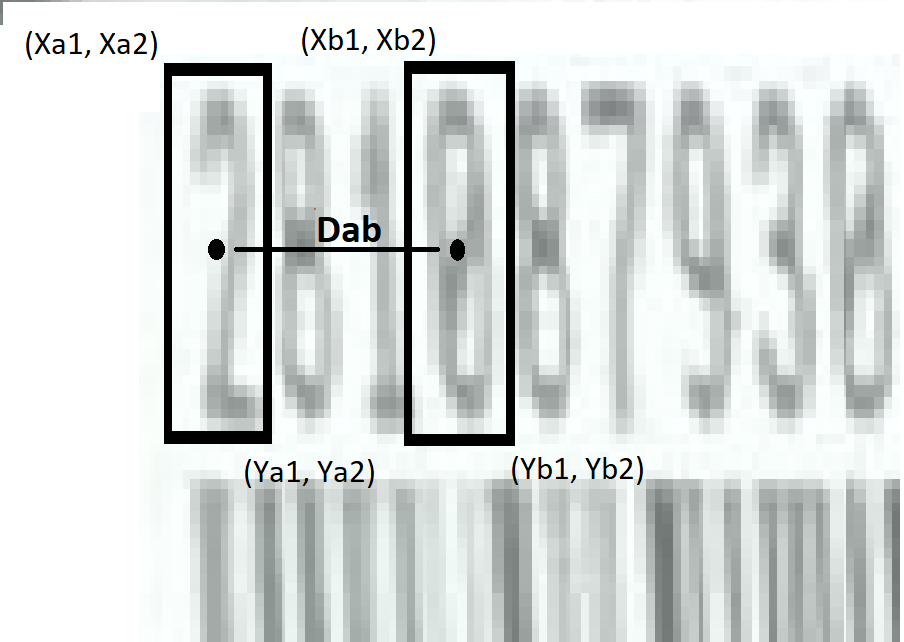
\includegraphics[width=0.6\linewidth]{figuras/MachineLearning/dab.png}
	\caption{Cálculo da distância entre dois números}
	\label{fig:dab}
\end{figure}

Calculo da coordenada central de cada região:
\begin{equation} 
ac = \left[\frac{(a_{x1} + a_{x2})}{2} \quad  \frac{(a_{y1} + a_{y2})}{2}\right] = [(a_{cx}\quad  a_{cy})]
\label{eq: central_a}
\end{equation}

\begin{equation} 
bc = \left[\frac{(b_{x1} + b_{x2})}{2} \quad  \frac{(b_{y1} + b_{y2})}{2}\right] = [(b_{cx}\quad  b_{cy})]
\label{eq: central_b}
\end{equation}


Distância entre coordenadas as centrais:
\begin{equation} 
Dab = \sqrt{(b_{cx} - a_{cx})^2 + (b_{cy} - a_{cy})^2}.
\label{eq: euclid}
\end{equation}

Ao identificar os números repetidos, escolhe-se o de maior acurácia para manter, pois quanto maior a acurácia, maior a probabilidade do número estar correto (Código \ref{ap:removeNumber}).
%
No final da execução do \textit{script} de remoção de números duplicados, verifica-se a quantidade de dígitos identificados na etiqueta, pois ainda podem existir números repetidos por estarem fora do parâmetro de comparação de distância entre os centros.

Caso haja mais de 13 dígitos, aqueles de menor acurácia são deletados até que restem 13 números (Código \ref{ap:identNumber}).

Para chamar atenção do usuário final a um possível erro de identificação, é gravada uma \textit{flag}
%
\footnote{Mecanismo lógico que funciona como semáforo: uma entidade (objeto) detém como ativa uma determinada \textit{flag} se a característica associada a essa \textit{flag} estiver presente.} 
%
de alerta em cada número da etiqueta que tenha acurácia menor que 98\%. Este aviso será mostrado pelo \textit{front-end}. 

O resultado da saída do modelo da rede neural de números é gravado em um arquivo "database.json", contendo os objetos detectados (números), a acurácia, a posição da bbox e a \textit{flag} de alerta de cada número (Figura \ref{fig:imageTag}).

\begin{figure}[H]
	\centering
	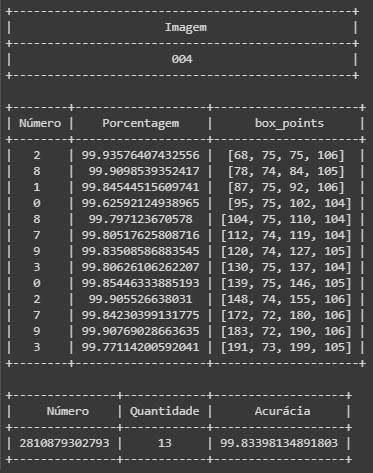
\includegraphics[width=0.53\linewidth]{figuras/MachineLearning/imageTag.png}
	\caption{\textit{Output} de uma das imagens do algoritmo de detecção de números.}
	\label{fig:imageTag}
\end{figure}

\section{Sistema Web}
O propósito desta aplicação é que a conferência das corridas pelo usuário final sejam facilitadas. Com o sistema web, ele terá um relatório detalhado e de forma automática os dados de cada corrida.
%
Nesta seção são apresentadas as etapas de desenvolvimento dos microsserviços utilizados no sistema elaborado, assim como o \textit{back-end} e o \textit{front-end}. 

\subsection*{Divisão dos arquivos}

Os microsserviços desenvolvidos foram projetados para seguir a \textit{Clean Architecture}. Esta arquitetura consiste em dividir as responsabilidades dentro de uma aplicação, encapsulando e abstraindo o código para facilitar a leitura e entendimento das funções de cada arquivo \cite{martin2000clean}. A Figura \ref{fig:cleanArchtecture} mostra a divisão dos arquivos utilizando a \textit{Clean Architecture} do Sistema Web.

\begin{figure}[htbp]
	\centering
	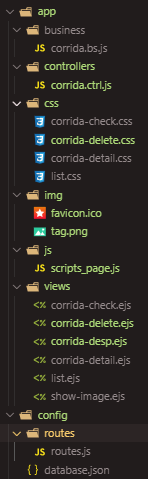
\includegraphics[width=0.22\linewidth]{figuras/WebService/cleanArchtecture.png}
	\caption{Divisão dos arquivos do Sistema Web}
	\label{fig:cleanArchtecture}
\end{figure}



Na pasta \textit{"/config/routes"} encontram-se as configuração das rotas utilizadas no sistema. Em \textit{controllers} é feito o tratamento dos \textit{inputs} e respostas das rotas, redirecionando para os \textit{business}, que é onde está a lógica principal da aplicação. No arquivo database.json é onde acontece a interação com o banco de dados. 
%
O \textit{front-end} da aplicação se encontra nas pastas css, js e views, sendo responsáveis pela interface gráfica do sistema.

\subsection{Back-end}

Esta seção trata da regra de negócio\footnote{Regra de negócio é a lógica que guia o comportamento e define "O que, onde, quando, por que e como" será feito, além de como o negócio será gerenciado ou governado.} do sistema, bem como a comunicação com banco de dados que estão gravados em arquivos JSON.

As operações são realizadas através dos \textit{endpoints}, que é uma forma de comunicação entre os sistemas. O sistema os disponibiliza como endereços para acesso, que podem receber e enviar informações, dependendo do que foi programado (Tabela \ref{tab:endpoints}).
%
A \textit{engine} EJS foi utilizada para que o \textit{back-end}, em Node.JS, comunique com \textit{front-end} através do consumo dos \textit{endpoints}, que significa enviar informações para estes \textit{endpoints}, esperando algum retorno, de sucesso ou falha.

\begin{table}[H]
	\centering
	\begin{tabular}{|l|l|}
		\hline
		\rowcolor[HTML]{ECF4FF} 
		\multicolumn{1}{|c|}{\cellcolor[HTML]{ECF4FF}\textit{Endpoint}} & \multicolumn{1}{c|}{\cellcolor[HTML]{ECF4FF}Característica} \\ \hline
		/ & \begin{tabular}[c]{@{}l@{}} retorna a lista de corridas existentes e redireciona\\ para \textit{home-page}\end{tabular}\\ \hline
		/corrida-detail & \begin{tabular}[c]{@{}l@{}}retorna os detalhes da corrida selecionada e redireciona\\ para tela \textit{corrida-detail}\end{tabular} \\ \hline
		/corrida-check & \begin{tabular}[c]{@{}l@{}} despacha a corrida e salva no banco de dados o\\ status "Despachada"\end{tabular} \\ \hline
		/corrida-delete & \begin{tabular}[c]{@{}l@{}} deleta a corrida e move seu arquivo "config\_x.json"\\ para pasta /deleted\\\end{tabular}\\ \hline
		/show-image & \begin{tabular}[c]{@{}l@{}}redireciona para tela de edição da etiqueta\end{tabular}\\ \hline
		/edit-image & possibilita a edição do número da etiqueta\\ \hline
		/upload-image & \begin{tabular}[c]{@{}l@{}}carrega uma foto para dar \textit{start} no sistema de \\detecção de objetos. \\\end{tabular}\\ \hline
	\end{tabular}
	\caption{\textit{Endpoints} do sistema WEB.}
	\label{tab:endpoints}
\end{table}

Os \textit{controllers} possuem módulos que são responsáveis pela renderização, navegação das paginas através dos \textit{endpoints}, bem como no envio de dados para o navegador.
%
Os \textit{business} são os responsáveis pelas regras de negócio do sistema de modo que cada método tenha uma função especifica. Suas principais funções são comunicação entre os aquivos JSON e listagem dos objetos.

\subsection{Front-end}

Nesta seção serão apresentadas as telas e suas funcionalidades utilizando o \textit{frontend} da aplicação. No desenvolvimento foram utilizadas as tecnologias HTML, CSS, JavaScript e para comunicação entre \textit{frontend} e \textit{backend}, o EJS.

A tela inicial do sistema é composta pela lista de corridas que já foram identificadas e pelo componente responsável por fazer o \textit{upload} de uma nova imagem (Figura \ref{fig:list1}).

A imagem será enviada para a pasta \textit{images} (Figura \ref{fig:folderSystem}) e automaticamente treinada pelo sistema de detecção.

Toda corrida que é inicialmente treinada terá o status de "Inadimplente" pois ainda não foi despachada para Laminações. Dessa forma, o sistema possui diversas opções para que o usuário tenha total controle da mesma.

A lista de corridas tem, como funcionalidade, as opções de visualizar detalhadamente ou deletar a corrida escolhida. Caso a corrida seja deletada, a tela será redirecionada para a página de \textit{delete} (Figura \ref{fig:corrida_delete}) e no \textit{backend} o arquivo config\_x.json é movido para pasta \textit{deleted} (Figura \ref{fig:folderSystem}).

\begin{figure}[H]
	\centering
	\includegraphics[width=1\linewidth]{figuras/WebService/Screens/list  1.png}
	\caption{Componente para \textit{upload} de novas imagens}
	\label{fig:list1}
\end{figure}

\begin{figure}[H]
	\centering
	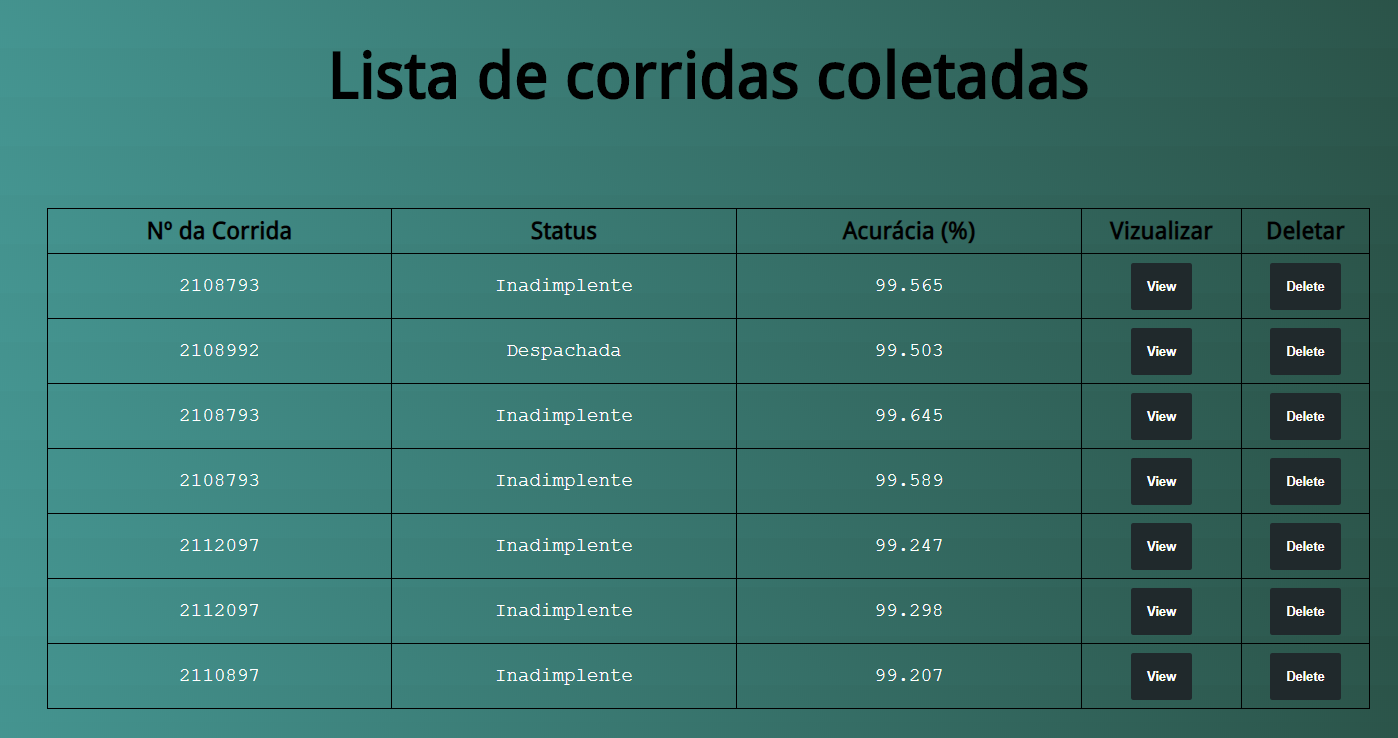
\includegraphics[width=1\linewidth]{figuras/WebService/Screens/list 2.png}
	\caption{Lista de corridas coletadas}
	\label{fig:list2}
\end{figure}

\begin{figure}[H]
	\centering
	
\includegraphics[width=0.5\linewidth]{figuras/WebService/Screens/corrida_delete.png}
	\caption{Corrida deletada.}
	\label{fig:corrida_delete}
\end{figure}

A segunda tela é o detalhamento da corrida selecionada em que é mostrado seu número, a quantidade de peças, a acurácia média das etiquetas e o status atual (Figura \ref{fig:detalCorrida}).

\begin{figure}[H]
	\centering
	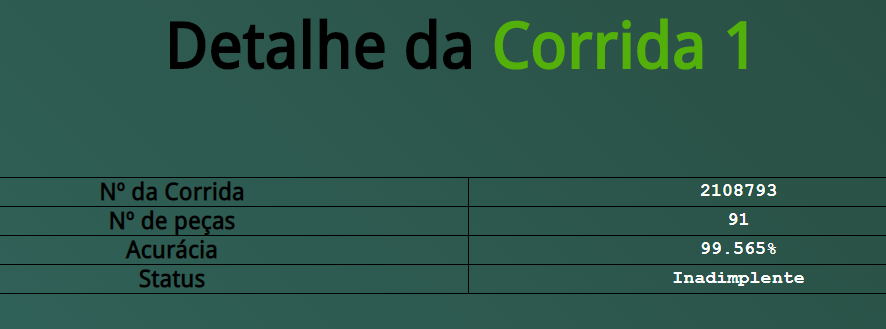
\includegraphics[width=0.7\linewidth]{figuras/WebService/Screens/detail 1.png}
	\caption{Detalhamento da corrida selecionada}
	\label{fig:detalCorrida}
\end{figure}

Ainda na tela de detalhamento, são mostradas todas as peças (etiquetas) que foram detectadas pelo sistema. A lista detalha o identificador, o número da peça que é referente ao número localizado acima do código de barras da etiqueta, a acurácia de identificação de cada dígito e um botão para visualizar a imagem da etiqueta (Figura \ref{fig:detail2.1}).

Caso algum algarismo tenha acurácia menor que 98\%, o fundo da cédula é preenchido pela cor vermelha, alertando ao usuário que o número identificado pode estar errado.

O botão despachar tem a função de alterar o status da corrida para "Despachada" no banco de dados (Figura \ref{fig:corrida_desp}) e assim deixá-la disponível para a Laminação. Caso o status da corrida já esteja como "Despachada", o sistema redirecionará o usuário para tela de erro como mostrado na Figura \ref{fig:corrida_desp_x}. 

\begin{figure}[H]
	\centering
	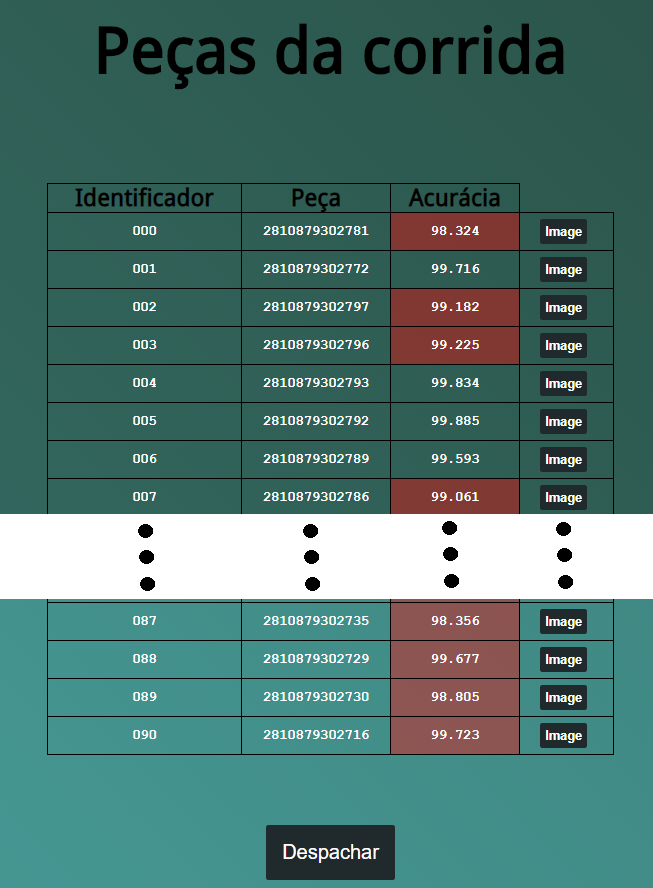
\includegraphics[width=0.65\linewidth]{figuras/WebService/Screens/detail 2.1.png}
	\caption{Detalhamento das peças da corrida}
	\label{fig:detail2.1}
\end{figure}

\begin{figure}[H]
	\centering
	
\includegraphics[width=0.5\linewidth]{figuras/WebService/Screens/corrida_desp.png}
	\caption{Corrida despachada pelo usuário}
	\label{fig:corrida_desp}
\end{figure}

\begin{figure}[H]
	\centering
	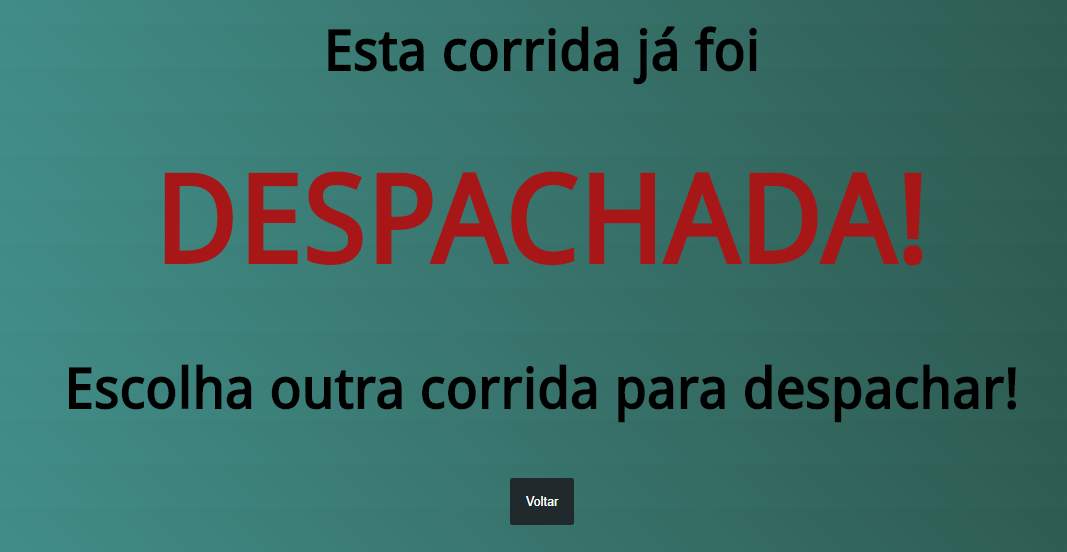
\includegraphics[width=0.5\linewidth]{figuras/WebService/Screens/corrida_desp_X.png}
	\caption{Mensagem de erro para status de corrida despachada}
	\label{fig:corrida_desp_x}
\end{figure}

A última tela do sistema é referente ao detalhamento da etiqueta que foi escolhida através do botão "\textit{Image}".

Nesta tela, o usuário terá permissão para editar a etiqueta caso tenha identificado algum algarismo erroneamente reconhecido.

Ao salvar, redireciona-se para tela de detalhamento da corrida para a continuidade do processo de verificação das demais etiquetas ou despache a corrida.

\begin{figure}[H]
	\centering
	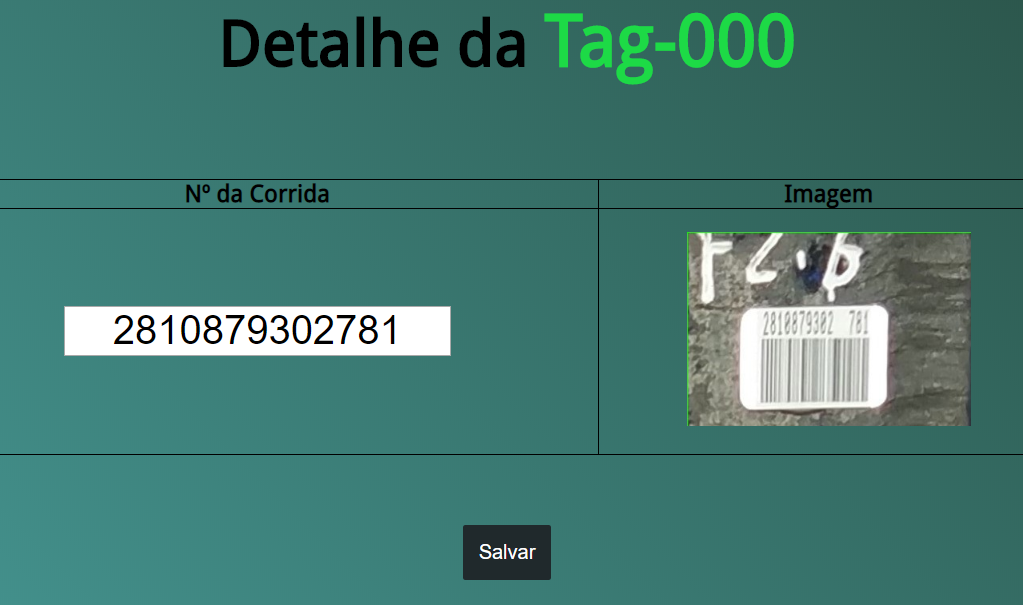
\includegraphics[width=0.8\linewidth]{figuras/WebService/Screens/detail_tag.png}
	\caption{Edição dos números da etiqueta.}
	\label{fig:detail_tag}
\end{figure}


Foi concluído que 99.05\% dos códigos de barras foram identificados corretamente e a Tabela \ref{tab:numberRecognize} mostra o resultado da porcentagem de acerto total de cada número detectado.


\begin{table}[H]
	\centering
	\begin{tabular}{|l|l|l|}
		\hline
		\rowcolor[HTML]{ECF4FF} 
		\multicolumn{1}{|c|}{\cellcolor[HTML]{ECF4FF}\textit{\textit{Número}}} &
		\multicolumn{1}{|c|}{\cellcolor[HTML]{ECF4FF}\textit{Porcentagem}}\\ \hline 
		0&  98.18\% \\ \hline
		1&  92.20\% \\ \hline
		2&  87.01\% \\ \hline
		3&  94.66\%\\ \hline
		4&  72.07\% \\ \hline
		5&  85.96\% \\ \hline
		6&  96.11\% \\ \hline
		7&  97.86\% \\ \hline
		8&  98.39\% \\ \hline
		9&  96.24\% \\ \hline
	\end{tabular}
	\caption{Assertividade dos números}
	\label{tab:numberRecognize}
\end{table}